\documentclass[11pt]{article}
\usepackage{geometry} % see geometry.pdf on how to lay out the page. There's lots.
\usepackage{hyperref}
\usepackage{graphicx}
\usepackage{gensymb}
\usepackage[affil-it]{authblk}
\usepackage[toc,page]{appendix}
\usepackage{pifont}
\usepackage{amsmath}
\usepackage{amsthm}

\usepackage{float}

\newtheorem{theorem}{Theorem}
\newtheorem{conjecture}{Conjecture}
\newtheorem{proofsketch}{Proof Sketech}
\usepackage{draftwatermark}

\SetWatermarkText{DRAFT}
\SetWatermarkScale{6}
\SetWatermarkLightness{0.95}

% \geometry{letter} % or letter or a5paper or ... etc
% \geometry{landscape} % rotated page geometry

% See the ``Article customise'' template for come common customisations

\title{A Continuum of Member-length Optimal Untwisted Boerdijk--Coxeter Helices}
\author{Robert L. Read
  \thanks{read.robert@gmail.com}
}
\affil{Founder, Public Invention, an educational non-profit.}


\date{\today}

%%% BEGIN DOCUMENT
\begin{document}

\maketitle

%% \tableofcontents

\begin{abstract}
  The Boerdijk--Coxeter helix (BC helix) is a face-to-face stack of regular tetrahedra whose outer vertices lie on helices.
  By using irregular tetrahedra, one can transform a BC helix, or tetrahelix, into a spaceframe that is not twisted, forming a novel object, a
  ``tetrabeam''.
  In the case of an equilateral profile, an analytic set of member lengths is provided which are shown to be optimal in minimize
  maximum lenghth difference, total member length, and sum of squared member lengths.
  This ``equitetrabeam'' is formed with only three member lengths ( two of $\sqrt{13/9}$, three are $\sqrt{10/9}$, and one of $1$.)
  It has 3-fold symmetry about  axis, and chirality.  
  A formula for the individual outer helices (and therby vertices) of the BC helix is given and
  unified with the formula for the equitetrabeam to create a continuum of ``untwisted'' BC helices optimal
  in the same senses mentioned above. This formula allows structures to in the continuum to be
  designed for pitch, curvature, torsion etc. by choice of $\lambda \in [0,1]$. Utility for truss/spaceframe design and
  robotics are discussed.
\end{abstract}


\section{Introduction}

The Boerdijk--Coxeter helix\cite{coxeter1985simplicial} (BC helix), also called the tetrahelix by Buckminster Fuller\cite{fuller1982synergetics}, is a stack of tetrahedra face to face that winds about a straight line. The vertices of the tetrahedra
lie upon three
helices about the central axes. The Tetrobot/Glussbot\cite{TetrobotBook} project
uses this regularity of this geometry to make a tentacle-like robot that can move like a slug or mollusc. The Tetrobot concept
is to use mechanical members, called actuators, which can change their length, connected by special joints which allow many
members to come to a single point. Such machines can follow purely mathematical models such as the Boerdijk–-Coxeter helix or the Octet Truss.

However, a tetrahelix does not rest on a plane in a simple way. It is convenient to have it ``untwist'' and form a spaceframe that
has a flat planar surface. By making length changes in a certain way, we can untwist a tetrahelix to form a ``tetrabeam'' which
is perfectly flat and has, for example, an equilateral triangular profile.

\section{Approach}

A tetrahelix has the useful property that every member is precisely the same length. If we relax this, so that the tetrahedra it
comprises are not perfectly regular, then we can twist and curve the tetrahelix into a variety of shapes. This is useful to
the mechanical engineer or robotocists because the structure remains an inherently rigid, omni-triangulated space frame, which
may be expected to be at least somewhat mechanically strong.

In particular, we can untwist the perfectly regular tetrahelix to form a ``tetrabeam''. We seek a tetrabeam that is irregular
(in terms of its tetrahedra) but regular enough in terms of mechanical engineering to be comprehensible and computationally tractable.
Observe that a regular tetrahelix appears to have three bumpy ``tracks'' which wind about the central axis.  We seek to unwind
these tracks so each track is a plane.

In order to do this for an tetrahelix of arbitrary length, we need a nameing convention for each member. We propose a coloring
scheme in which the joints and members on the outer ``rails'' of the tetrahelix are colored in primary colors red, yellow and blue.
We propse that the interior members be colored based on the rails they connect using an additive color scheme, or orange, purple, and green,
if the member connects red to yellow, red to blue, or blue to yellow, respectively.  Furthermore, we call interor members ``even'' if they
are even numbered starting from the joint at the origin, and ``odd'' if they are odd-numbered.  We have found that nine classes thus
formed are sufficient to untwist the tetrahelix and for our purposes: $red, yellow, orange_{even}, orange_o, purple_e, purple_o, green_e, green_o$. In the diagram below, the ``odd'' members are draw with a dashed line.


 \begin{figure}[H]
     \centering
     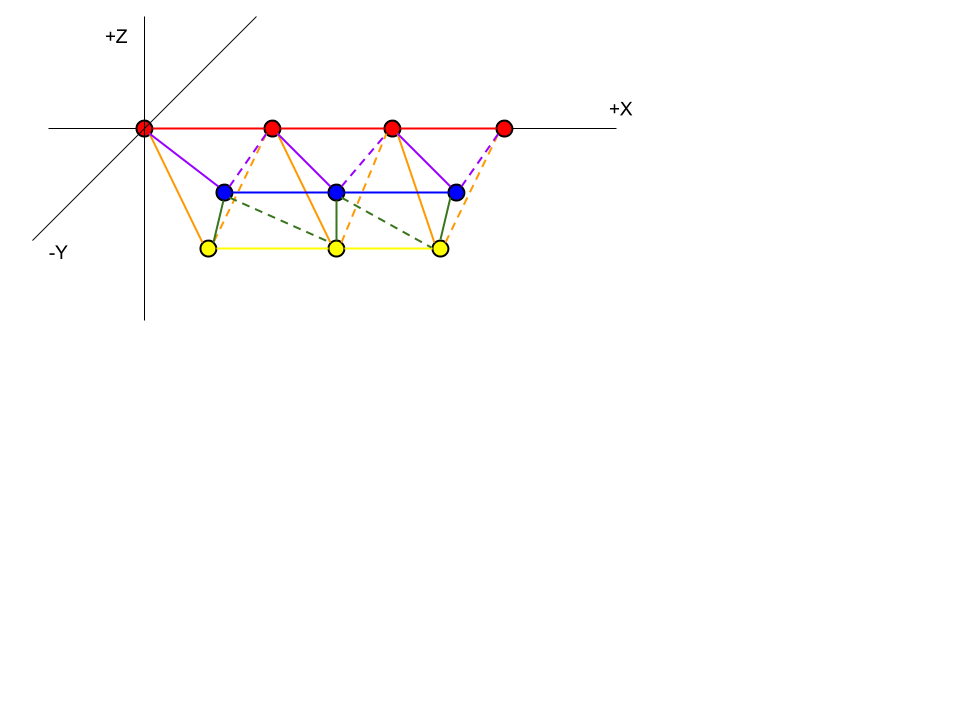
\includegraphics[width=0.9\textwidth]{TetrahelixColoringDiagram.png}
     \caption{Coloring of an (untwisted) Tetrabeam}
 \end{figure}

 Having observed that the tetrahelix can form a tetrabeam, we need merely compute the length of the member classes.

 Although one could choose any beam width and beam height in principle, and a structural engineer would like choose a ``deep'' beam that had
 a height greater than its width, our primary motivation is support the Tetrobot, which uses members that all have the same maximum and
 minimum length. It therefore is sensible to consider a ``tetrabeam'' with the cross-sectional profile of an equilateral triangle.
 Furthermore, acting as robotics engineers we seek to have all members to be similar in length, because this allows us the greatest
 flexibility in making the tetrabeam crawl, or walk, or curl, topics outside the scope of this paper.

 If we simply constrain all red joints to the origin and all blue joints to a line parallel to the x-axis at the vertix of an equilateral
 triangle descending from the origin, we will have simple equations in Cartesian space. We use the variable B to mean the x coordinate
 of the $blue_0$ node and Y to mean the x-coordinate of the $yellow_0$ node. Since for our purposes we do not need distance but rather relative distances
 until our last step, we organize these equations as \emph{quadrances}, leaving both sides of the equations squared.
 We further assume the red, yellow and blue members are all unity. The alitude of an equilateral triangle is $\sqrt{3}/2$.
 These equations follow from the distance formula in three space.
 \begin{align*}
   D^2 &= (\Delta z)^2 + (\Delta y)^2 + (\Delta x)^2 \\
 orange_e^2 &= (\sqrt{3}/2)^2 + (1/2)^2 + Y^2 & &= 1 + Y^2\\
 orange_o^2 &= (\sqrt{3}/2)^2 + (1/2)^2 + (1-Y)^2 & &= 1 + (1-Y)^2\\
 purple_e^2 &= (\sqrt{3}/2)^2 + (1/2)^2 + B^2 & &= 1 + B^2\\
 purple_o^2 &= (\sqrt{3}/2)^2 + (1/2)^2 + (1-B)^2 & &=  1+ (1-B)^2\\
 green_e^2 &= (B - Y)^2 + 1^2 + 0^2 & &= 1 + (B - Y)^2 \\ 
 green_o^2 &= ((1+Y) - B)^2 + 1^2 + 0^2 & &= 1 + ((1+Y) - B)^2 \\ 
\end{align*}

 We then ask the question: what are useful values for B and Y, from which we will have constrained and computed the lengths of all
 members.

 \section{Choosing the parameters}

 Choices of $Y$ and $B$ correspond to slideing the yellow and blue rail relative to the red rail. However, we seek to choose them such that all
 classes of members have similar lengths. In particular, we want to minimize the difference between the shortest and longest.

 It particular we have no interest in solutions in which these rails swing past the $red_1$, or swing behind $red_0$, so we
 assert $0 \leq Y \leq 1$ and $0 \leq B \leq 1$. Without loss of generality, let us choose that $Y$ will be the at least as close to the origin as $B$,
 so $Y  < B$.

 We investigate possible choices of $Y$ and $B$ numerically with a computer before observing the apparent result that the maximum distance in
 length is minimized when $Y = 1/3$ and $B = 2/3$.

 \begin{theorem}
A Tetrabeam of mininimum maximum difference between edge lengths is formed when $Y = 1/3$ and $B = 2/3$.
\end{theorem}

 \begin{proof}
   First we show that asserting $Y + B = 1$ does not worsen our solution.

   Assume $Y'' = Y' + k, B'' = B' + k$, where $k > 0$. Algebraically, subsituting $Y'', B''$ into the equations for the $green$
   classes above does not change them. Geometrically, swinging  the yellow or blue rail by the same amount does not change the
   shape of the green triangles. Therefore we may choose the sum $ Y+B $ to be whatever we want without increasing the length
   of $green_e$ or $green_o$.

   By assume, $Y < B$, therefore $orange_e < purple_e$ and $orange_o > purple_o$. $Y$ cannot be greater than $1/2$, because
   if it were we could shorten the longest member $purple_e$ by lowering both $Y$ and $B$. Therefore $orange_e < orange_o$.
   Similarly $purple_o < purple_e$. So $orange_e$ and $purple_o$ cannot be the longest members of the four.

   Of the four remaining member lengths, suppose that $orange_o$ or $purple_e$ is one of the longest. Whichever it is can ben be shortened
   until it is equal to the other, or:
 \begin{align*}
 orange_o^2  &= 1 + (1-Y)^2 & &=  purple_e^2  &= 1 + B^2\\
 \end{align*}
 or, by algebra,
 \begin{align*}
   1 + (1-Y)^2 &= 1 + B^2\\
   (1-Y)^2 &= B^2\\
 \end{align*}
 which is solved by $Y+B = 1$.

 Thus an optimal minimax solution will have $orange_o = purple_e$ and $orange_e = purple_o$, and $Y+B = 1$.
 (Note: Although these classes are the same for the purpose of the Equitetrabeam, for other purposes of robotics
 they may not be. We therefore retain our color naming scheme.)

 We now need only choose $Y$ so as to miniize these two classes against the $green$ class.

   Assume that $Y \leq 1/2$. Then $B \geq 1/2$. Substituing $1 - Y$ for $B$ in our equations:
 \begin{align*}
   orange_e^2 &= 1 + Y^2 \\
 orange_o^2 &= 1 + (1-Y)^2 \\
 purple_e^2 &=  1 + (1-Y)^2 \\
 purple_o^2 &=   1+ (1-B)^2 & &= (1 + (1 - (1 - Y))^2 & & = 1 + Y^2 \\
 green_e^2 &=  1 + (B - Y)^2 & &= (1 - ((1 - Y - Y)^2)) & &= 1 + (1 - 2Y)^2\\ 
 green_o^2 &= 1 + ((1+Y) - B)^2 & &= 1 + ((1+Y) - (1 - Y))^2 & &= 1 + (2Y)^2 \\
 \end{align*}

 By graph inspection we observe that $green_o$ > $green_e$ for $Y > 1/4$ and $green_e < orange_o$ for $Y < 2/3$.

 For the case $Y < 1/4$, $green_o < green_e < orange_o$. Because $Y \leq 1/2$, $orange_e < orange_o$. So $orange_o$
 is the longest member, and its length increases as $Y$ goes to $0$. So at $Y = 1/4$, $orange_o$ attains its
 minimum value of:
\begin{align*}
 orange_o^2 &= 1 + (1-Y)^2 \\
 orange_o^2 &\geq 1 + (1-1/4)^2 \\
 orange_o^2 &\geq 1 + (3/4)^2 \\
 orange_o^2 &\geq 1 + 9/16 \\
 orange_o &\geq \sqrt{25/16} \\
    orange_o &\geq 5/4 \\ 
 \end{align*}
  
For the case $Y >= 1/4$, $green_o$ and $orange_o$ are the two largest of these values, so that
we minimize the entire group by setting them equal.
 Then:
\begin{align*}
  green_o^2 &= orange_o^2 \\
  1 + (2Y)^2 &= 1 + (1-Y)^2 \\
  4Y^2 = 1 + -2Y + Y^2 \\
  3Y^2 + 2Y - 1 = 0 \\
\end{align*}
Which has two solutions, one of which is $Y = -1$, which we throw out because we assumed $0 \leq Y$. The other is $Y = 1/3$.

Therefore $Y = 1/3$ minimizes the length difference of all members.


Our complete solution is therefore:
\begin{align*}
  Y &= 1/3 \\
  B &= 2/3 \\  
   orange_e &= \sqrt{1 + (1/3)^2} & &= \sqrt{10/9} \\
 orange_o &= \sqrt{1 + (1-1/3)^2} & &= \sqrt{13/9} \\
 purple_e &=  orange_o  \\
 purple_o &=  orange_e \\
 green_e &=  \sqrt{ 1 + (1 - 2/3)^2} & &= \sqrt{10/9} \\ 
 green_o &=  \sqrt{1 + (2/3)^2} & &= \sqrt{13/9} \\
\end{align*}

Since $\sqrt{13/9} < 5/4$ the solution $Y = 1/3$ is better than $Y = 1/4$.

 \end{proof}

So in fact we can construct a tetrabeam using only three member lengths $1$,
$\sqrt{10/9} = 1.05409\cdots$, and $\sqrt{13/9} = 1.20185\cdots$.
In other words, our longest members is only 21\% longer than our shortest member.
As it happens, the current Tetrobot implementation can support about a 50\%
change in length, so it can easily realize this Tetrabeam configuration. If one were
to construct a static tetrabeam by welding, this limited number of member lengths would be convenient.

\section{Additional Properties of the Equitetrabeam}

The irregular tetrahedron $ABCD$ of edge lengths $AD = 1, AB = BC = CD = \sqrt{10/9}, AC = BD = \sqrt{10/9}$ stacks
such that three together form a oblique equilateral prism of parallel base faces. Such prism stack linearly into
a prism of any length. If we imagine a long prism made of many cells, there is one node at each 1/3rd of a unit length
along the axis. The cross-sectional face of the equitetrabeam is an equilateral triangle, although none of the faces
are.

\begin{theorem}
  The Equitetrabeam is also optimal under the metric of the sum of the squares of all members
  for an equilateral tetrabream isomorphic to the Boerdijk--Coxeter helix.
  \end{theorem}

\begin{proof}
  Summing together all 6 squared lengths:
\begin{align*}
  sum &= orange_e^2 + orange_o^2 + purple_e^2 + purple_e^2 + purple_o^2 + green_e^2 + green_o^2 \\
   &= 1 + Y^2 + 1 + (1-Y)^2 +  1 + B^2 +  1+ (1-B)^2 + 1 + (B - Y)^2 + 1 + ((1+Y) - B)^2 
\end{align*}
  creates expression most easily minimized with Wolfram Alpha, which gives:
\begin{align*}
min\{1 + Y^2 1 + (1 - Y)^2 + 1 + B^2 + 1 + (1 - B)^2 + 1 + (B - Y)^2 \\
  + 1 + ((1 + Y) - B)^2\} = 20/3 \\
at (B, Y) = (2/3, 1/3)
\end{align*}
  
\end{proof}

\begin{theorem}
  The Equitetrabeam is also optimal under the metric of the total length of all members 
  for an equilateral tetrabream isomorphic to the Boerdijk--Coxeter helix.
\end{theorem}

\begin{proof}
  Summing together all lengths:
  \begin{align*}
  sum &= orange_e + orange_o + purple_e + purple_e + purple_o + green_e + green_o \\    
  &= \sqrt{1 + Y^2} + \sqrt{1 + (1-Y)^2} + \sqrt{1 + B^2} + \sqrt{1+ (1-B)^2} + \\
  & \sqrt{1 + (B - Y)^2} +  \sqrt{1 + ((1+Y) - B)^2} \\
  \end{align*} 

  Wolfram Alpha, evaluating this numerically, gives the same minima:
  
  \begin{tabular}{c}    
$  min\{\sqrt(1 + Y^2) + \sqrt{1 + (1 - Y)^2} + \sqrt{1 + B^2} + \sqrt{1 + (1 - B)^2} + $\\
    $  \sqrt{1 + (B - Y)^2} + \sqrt{1 + ((1 + Y) - B)^2}\} $ \\
    $ \approx 6.76783 \text{at } (B, Y) \approx (0.666667, 0.333333) $
  \end{tabular}

  
\end{proof}

The equitetrabeam has chirality.

\section{The Rail Helices}

If you can choose member lengths, you can form a linear combination of the equitetrabream lengths and the completely regular
lengths of the tetrahelix, thereby choosing the torsion.  If you are designing a spaceframe, this is a static design choice,
in a robot, it is a dynamic choice that can be used to twist the robot and/or exert torsion on the environment.

Ideally we would have a simple formula for defining the nodes based on any torsion we choose.
Unfortunately, it is not obvious that a linear combination of lengths produces a simple formular.
It is a goal of this paper to relate these two approaches to generating a tetrahelix continnum.

H. S. M. Coxeter constructs the Tetrahelix as a repeated rotation and translation of the tetrahedra, showing the
rotation is:
\[
\theta = \arccos(-2/3) 
\]
and the translation:
\[
h_{bc} = 1/\sqrt{10}
\]


$\theta$ is approximately $131.8103149$ degrees.
The angle $\theta$ is the rotation of a \emph{each} tetrahedra.
That is, a yellow tetrahedron is rotated slightly more than a $1/3$ of a revolution to match the face of the red tetrahedra.
$3 \theta - 2\pi$ is the apparent roation of $V_3$ relative to $V_0$.

From Robert Gray's site, repeating formula by H.S.M. Coxeter:
\[
V_n =
\left [
  \begin{tabular}{c}
   $ r_{bc} \cos(n \theta $\\
   $ r_{bc} \sin(n \theta) $\\
   $ n h_{bc}  $
  \end{tabular}
\right ]  
\]
where:
\[
r_{bc} = \frac{3\sqrt{3}}{10} 
\]
and where $n$ represents each integer numbered node in succession. That is, in our coloring scheme, $V_0$ is red, and$ V_1$ is yellow,  $V_2$ is blue,
$V_3$ is red, etc. 

This formula defines a helix, but it is not any of the helices of the Tetrahelix, but rather one that winds three times
as rapidly through all nodes. However, it is convenient to have a formula that gives us the nodes of just
each colored helix. Such a helix can be written:

\[
H_{BCcolored}(n,c) =
\left [
  \begin{tabular}{c}
   $ r_{bc}  \cos((3 \theta - 2 \pi)n + c  \theta $\\
   $ r_{bc} \sin((3 \theta - 2 \pi)n + c  \theta $\\
   $ (n + c/3) 3  h_{bc} $
  \end{tabular}
\right ]
\]
where $c \in \{0,1,2\}$ to represent red, yellow, or blue.

In this formula, $n$ may be taken as a node number for one rail. Allowing $n$ to take non-integer values defines a continuous
helix in space which is close to the segmented polyline of the outer tetrahedra edges, and coincides with them at integer
values.
The quantity $ (3 \theta - 2 \pi) \approx 35.43 \degree $, and is the approximate angular shift between $V(n,color)$ and
$V(n+1,color)$. This quantity appears so often below that we call it the ``rail angle rho'', $\rho = (3 \theta - 2 \pi)$.
Since:
\[ \frac{2 \pi}{\rho} \approx 10.1606....
\]
We can see that there are approximately $10.16$ red, blue or yellow tetrahedra on one rail in a single revolution.
The pitch of the Boerdijk--Coxeter helix of edge length $1$ is the length of three tetrahedra times this number:
\begin{align*}
  &= \frac{2 \cdot 3 \pi h}{\rho} \\
  &= \frac{3  \sqrt{\frac{2}{5}}  \pi}{\rho} \\
  &\approx 9.6392... \\
\end{align*}
The pitch is less than the number of tetrahedra because the tetrahedra are not lined up perfectly.

\section{Adding an Untwisting Parameter}

We observe that it by thinking of the straight lines of the Equitetrabeam as a degenerate helix of zero curvature,
it should be possible to define a smoothly varying continuum between the Boerdijk--Coxeter helix and the Equitetrabeam and every
curvature and torsion betwen the two.

This formulation $V(n,c)$ above is valuable, but obscures the essentially fact that the red, yellow, and blue helices are 120 degree rotations
of each other. In order to rewrite this expression with an explict rotation of $2\pi/3$, we expand 
the expression and seek to isolate the term $c2\pi/3$. (This took some searching.)
\begin{align*}
  \rho n + c \theta  &=   \text{\{we aim for 3 in denom, so we split...\}} \\
    (3 \theta - 2 \pi)n + (c/3)  (\theta /3)  &=   \text{\{we want $2\pi$ in numerator, so add canceling terms...\}} \\
  (3 \theta - 2 \pi)n + (c/ 3) (3 \theta - 2 \pi  + 2 \pi) &=  \text{\{associate...\}} \\
  (3 \theta - 2 \pi)n + (c/ 3) ((3 \theta - 2 \pi)  + 2 \pi) &=  \text{\{distribute...\}} \\  
  (3 \theta - 2 \pi)n + (c / 3) (3 \theta - 2 \pi)  + c 2 \pi /3 &=  \text{\{collect like factors...\}} \\
  \rho (n + c/3)  + c 2 \pi /3  \\
\end{align*}
Now the the formula on the left is the only one that depends on the scalar $n$. We use this to a create
a new formulation $H_{symmetric}(n,c) = H_{colored}(n,c)$

\[
H_{BCsymmmetric}(n,c) =
\left [
  \begin{tabular}{c}
   $ r  \cos((\rho)(n + c/3)  + c 2 \pi /3) $\\
   $ r  \sin((\rho)(n + c/3)  + c 2 \pi /3) $\\
   $ (n + c/3) 3  h $
  \end{tabular}
\right ]
\]

We seek to unify this with degenerate helix formula for the equitetrabeam:
\[
H_{beam}(n,c) =
\left [
  \begin{tabular}{c}
   $ r_{etb}  \cos( 0 \cdot (n + c/3)  + c 2 \pi /3) $\\
   $ r_{etb}  \sin( 0 \cdot (n + c/3)  + c 2 \pi /3) $\\
   $ (n + c/3) h_{etb} $
  \end{tabular}
\right ]  
\]
where $ r_{etb} = 1/\sqrt(3)$, $h_{etb} = 1/3$,

Now basic components of the helix, which are the radius $r$, the rate of rotation $(\rho)(n + c/3)$, and the rate of
axial growth $ (n + c/3) 3  h $ can all be linearly interpolated with a parameter $\lambda$ between their high values (for the BC helix)
and low values (for the equitetrabeam):

\begin{align*}
r_{\lambda}  &=  \lambda (3 \sqrt(3) / 10 - 1/\sqrt(3)) +  1/\sqrt(3) \\
h_{\lambda} &=   \lambda (3 / \sqrt(10) - 1)+ 1 \\
rot_{\lambda} &=  \lambda \rho  \\
\end{align*}
to create a formula that generates a continuum of tetrahedral structures:

\[
H_{continnum}(n,c,\lambda) =
\left [
  \begin{tabular}{c}
   $ r_{\lambda} \cos(rot_{\lambda} (n + c/3) + c 2 \pi /3) $\\
   $ r_{\lambda}  \sin(rot_{\lambda} (n + c/3) + c 2 \pi /3) $\\
   $ h_{\lambda} (n + c/3) + 0 $
  \end{tabular}
\right ]
\]
A value of $\lambda = 0$ generates the Equitetrabeam, and $\lambda = 1$ generates the Boerdijk--Coxeter helix, and every
value $\lambda \in [0,1]$ generates an attractive structure which if physcially realized is an inherently rigid structure
with member lengths of no greater disparity than $21\%$.
In the sense of structureal engineering, it would be a relatively strong spaceframe.

Furhtermore, this formula allows one to design the pitch (in edge length units) as a function of $\lambda$ of the helix (along one rail)
where $\lambda \neq 0$:
\[
p(\lambda) = 2 \pi  \cdot \frac{((3/\sqrt(10) -1) \lambda +1)}{ \lambda  \rho }
\]


\section{Utility for Robotics}

Trusses and spaceframes remain an important design field in mechanical and structural enginnering\cite{mikulas1985sequentially},
including deployable and moving trusses\cite{claypool2012readily}.

Starting twenty years ago, Sanderson\cite{sanderson1996modular}, Hamlin,\cite{TetrobotBook}, and others including Lee\cite{lee2002dynamic}
created a style of robotics based on changing the lengths of members
joined at the center of a joint, thereby creating a connection to pure geometry. More recently NASA has experimented with
tensegrities\cite{NTRT}, a different point in the same design spectrum. These fields create a need to explore the notion of
geometries changing over time, not generally considered directly by pure geometry.

As suggested by Buckminster Fuller, the most convenient geometries to consider are those that have regular member
lengths, in order to facilitate the inexpensive manufacture and construction of the robot.  In a plane, the octest truss
is such a geometry, but in a line, the Boerdijk--Coxeter helix is a regular structure.

However, a robot must move, and so it is interesting to consider the transmuations of these geometries, which was in
fact the motivation for creating the equitetrabream.

\begin{theorem}

  Using the six member classes defined by the non-primary colors, it is possible to smoothly twist and untwist a tetrahelix by
  using a linear combination of lengths.
  
\end{theorem}

\begin{proof}
  Proof by our computer program that does this by forming a linear interpolation of links.
\end{proof}

\begin{figure}[H] %float with two figures
  \centering
     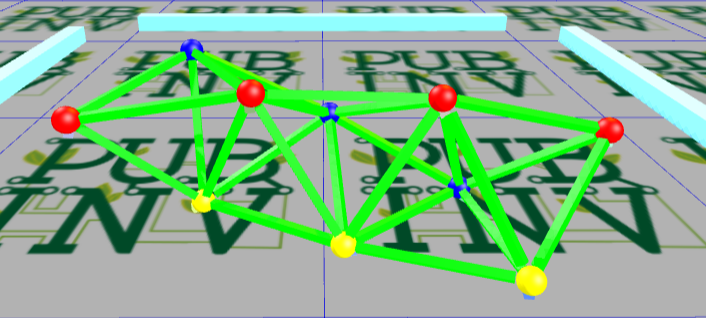
\includegraphics[width=0.4\textwidth]{figures/Tetrahelix0.png}
     \caption{Regular Tetrahelix}
     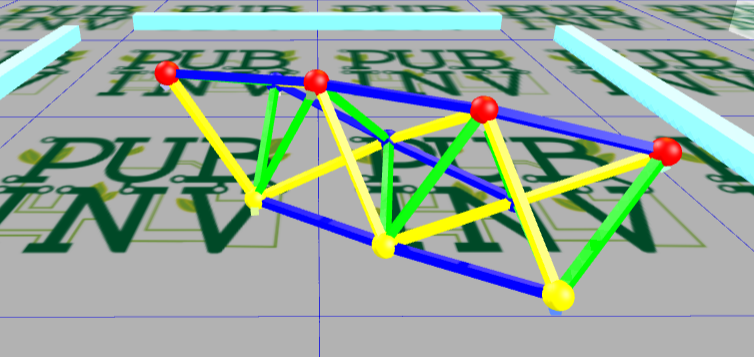
\includegraphics[width=0.4\textwidth]{figures/Tetrahelix1.png}
     \caption{2/3rd Twisted Tetrahelix}
     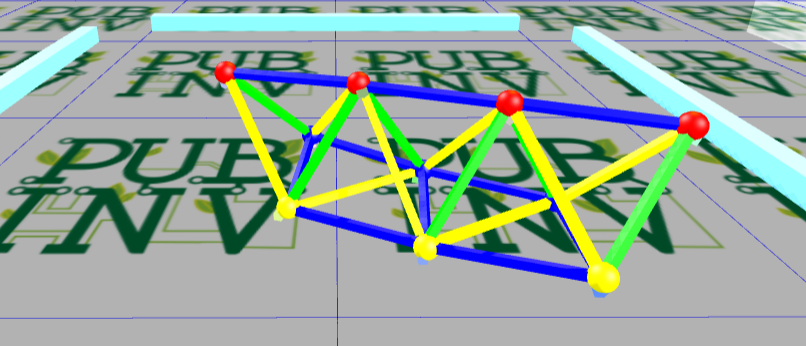
\includegraphics[width=0.4\textwidth]{figures/Tetrahelix2.png}
     \caption{1/3rd Twisted, 2/3rd Untwisted Tetrahelix}
     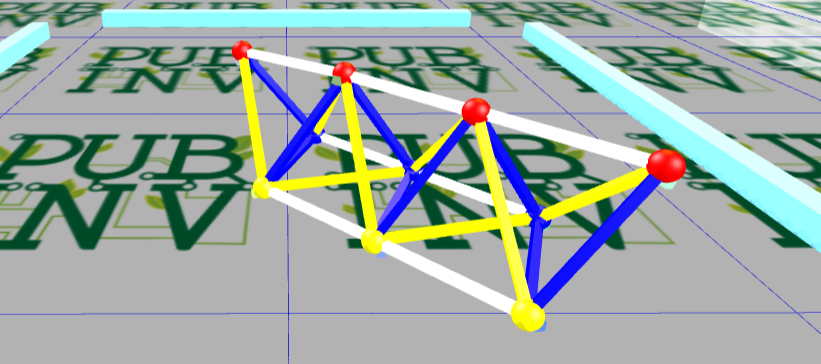
\includegraphics[width=0.4\textwidth]{figures/Tetrahelix3.png}
     \caption{The Equitetrabream: Fully Untwisted Tetrahelix}
\end{figure}

\section{Contact and Getting Involved}

The Gluss Project \url{http://pubinv.github.io/gluss/}
is a free-libre, open-source research, hardware, and software project that welcomes volunteers.
It is our goal to organize projects for the benefit of all humanity without seeking profit or intellectual property.
To assist, contact \href{mailto:read.robert@gmail.com}{$<$read.robert@gmail.com$>$}.

\bibliographystyle{IEEEtran}
\bibliography{IEEEabrv,gluss}

\end{document}

  Best reference is from Coxeter:
  
  http://cms.math.ca/openaccess/cmb/v28/cmb1985v28.0385-0393.pdf

https://arxiv.org/pdf/1302.1174.pdf
